\documentclass[../main.tex]{subfiles}

\graphicspath{{../image/}{../figure/}}

\begin{document}

\chapter{连续潜变量}\label{chapter:ch16-连续潜变量}

在\cref{chapter:ch15-离散潜变量}中，我们讨论了拥有离散潜变量的概率模型，例如 Gauss 混合模型。本章探讨部分或全部潜变量为连续变量的模型。研究这类模型的一个重要原因是很多数据集都有这样的特点：数据点都挤在一个比起原始数据空间维度低得多的流形（manifold）上。为什么会这样呢？想象一下，假如我们从 MNIST 数据集（LeCun et al., 1998）里选出一个显示手写数字的 $64\times64$ 像素灰度图，将它嵌入一个更大的 $100\times100$ 像素的图像中，图像边缘用数值为零的像素（对应白色像素）填充。嵌入的同时，随机改变数字的位置和方向，就像\cref{figure:ch16-合成数字数据集}展示的那样，那么每一个生成的图像由高达 10000 维（因为是 $100\times100$ 像素）的数据空间中的一个数据点来表示。然而在这样的图像数据集中，仅有三个自由度（degree of freedom）的变化，分别对应于垂直移动、平移及旋转。因此，这些数据点实际上存在于一个内在维度（intrinsic dimensionality）为 $3$ 的子空间中。请注意，这个流形是非线性的，因为如果我们将数字平移经过一个特定像素，那么这个像素的值将从 $0$（白色）变成 $1$（黑色），然后再变回 $0$，这显然是关于数字位置的非线性函数。在这个例子中，平移和旋转的相关参数是潜变量，因为我们只观察到图像向量本身，而不知道用来生成它们的平移或旋转变量的具体值。

\begin{figure}[htbp]
  \centering
  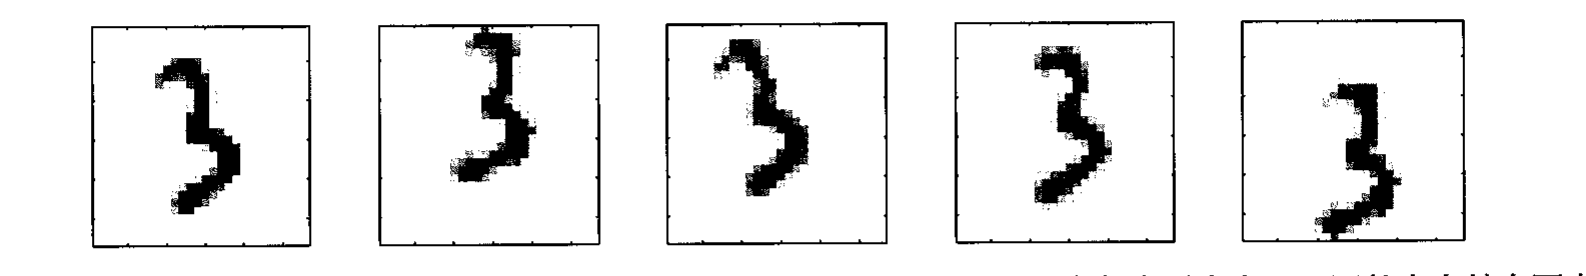
\includegraphics[width=0.95\textwidth]{ch16-fig16.1-digits-dataset.png}
  \caption{一个合成的数据集，从中获取一个手写数字图像并创建多个副本，在每个副本中，手写数字在某个更大的图像区域内进行随机移动和旋转}
  \label{figure:ch16-合成数字数据集}
\end{figure}

在真实的手写数字数据集中，会有更多的自由度出现。例如，不同人的书写风格有差异，而同一个人的书写风格也有变化，这就会导致手写数字在尺寸和其他方面上的变化。不过，即使有这些自由度，它们的数量相较于整个数据集的维度还是显得很少。

在实践中，数据点不会精确地局限于一个光滑的低维流形上，我们可以将数据点偏离流形的现象解释为“噪声”。我们可以自然地从生成性视角（generative view）来理解此类模型。首先根据某种潜变量分布在流形内选择一个点，然后添加从给定潜变量的数据变量的某种条件分布中抽取的噪声，生成一个观测数据点。

对于最简单的连续潜变量模型（continuous latent-variable model），可以假设潜变量和观测变量都遵循 Gauss 分布，并利用线性-Gauss 依赖性（linear-Gaussian dependence）（见\cref{subsection:ch11-Gauss变量}）来描述观测变量对潜变量状态的依赖。这引出了著名的主成分分析（Principal Component Analysis, PCA）概率公式，还有称为因子分析（factor analysis）的相关模型。本章首先介绍如何使用标准非概率方法来实现 PCA，随后揭示 PCA 如何自然而然地对应于线性-Gauss 潜变量模型的最大似然解（maximum likelihood solution）（见\cref{subsection:ch16-最大似然法}）。这种概率化表述带来了许多优势（见\cref{section:ch16-概率潜变量}），比如使用 EM 算法进行参数估计，规范化地扩展成 PCA 混合模型，以及通过 Bayes 公式自动从数据中确定主成分的数量（Bishop, 2006）。本章还为我们学习具有连续潜变量的非线性模型奠定了基础，这些模型包括标准化流、变分自编码器和扩散模型。

\subfile{Chapter-16/section-01.tex}
\subfile{Chapter-16/section-02.tex}
\subfile{Chapter-16/section-03.tex}
\subfile{Chapter-16/section-04.tex}
\subfile{Chapter-16/section-05.tex}

\end{document}
